% vim: set spell spelllang=es syntax=tex :

\documentclass[11pt,a4paper,spanish]{beamer}

\usepackage[spanish]{babel}

\usepackage[utf8]{inputenc}

\usepackage{graphicx}

\usepackage{subcaption} %Para Subfigure

\usepackage{caption} %Para captions en las figuras sin prefijo

\usepackage{ccicons}

\usepackage{url}

\usepackage{babelbib}

\usepackage{textcomp}

\usepackage{styles/egyptian}

\newcommand{\aprox}{\raisebox{0.5ex}{\texttildelow}}

\usefonttheme{serif}

\setlength{\parskip}{1.5mm}

\usetheme{Rochester}
\usecolortheme{whale}

%\usetheme{Warsaw}

\beamertemplatenavigationsymbolsempty

\setbeamertemplate{background canvas}{
    \raisebox{-0.99\paperheight}[0pt][0pt]{
        \makebox[\paperwidth]{
            \null
            \hspace{-1em}
            
\includegraphics[width=0.09\paperwidth]{logos/fai.pdf}
            \hspace{0.8\paperwidth}
            \hspace{-0.5em}
            \includegraphics[width=0.09\paperwidth]{logos/uncoma.pdf}
            }
    }
}

\title{Sistemas de numeración}

\author{}

\date{}

\defbeamertemplate{footline}{centered page number}
{
    \hspace*{\fill}
    \usebeamercolor[fg]{blue}
    \usebeamerfont{page number in head/foot}
    \insertpagenumber\,/\,\insertpresentationendpage
    \hspace*{\fill}\vskip2pt
}
\setbeamertemplate{footline}[centered page number]

\begin{document}

\begin{frame}[noframenumbering]

    \maketitle
    \centering
    \vspace{-8em}~
    \begin{figure}
    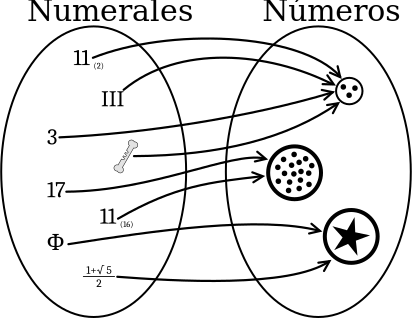
\includegraphics[height=0.65\textheight]{img/numerales.pdf}
        \captionsetup{textfont=tiny,labelformat=empty,justification=centering}
        \caption{}
    \end{figure}

\end{frame}

\begin{frame}

    \frametitle{Temario}

\begin{itemize}

    \item Números y numerales.

    \item Sistemas no posicionales.

    \item Sistemas posicionales:
    \begin{itemize}
        \item Conversión entre bases.
    \end{itemize}

\end{itemize}
\end{frame}

\begin{frame}

\frametitle{Números y numerales}

\begin{figure}
    \centering
    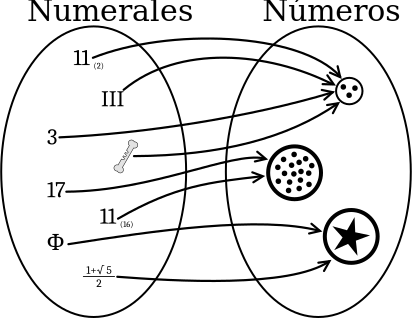
\includegraphics[height=0.9\textheight]{img/numerales.pdf}
    \captionsetup{textfont=tiny,labelformat=empty}
    \caption{}
\end{figure}

\end{frame}

\begin{frame}

\frametitle{Números y numerales}

\begin{itemize}
    \item Un numeral es la forma en la que representamos a un número.
    \item Los números son los conceptos abstractos que se pueden representar
        de múltiples formas y tienen propiedades intrínsecas independientes de
        esta.
\end{itemize}
\pause
\textbf{¿Es 42 número o numeral?}
\pause

\begin{itemize}
    \item La cadena de texto $4$ seguida de $2$ es el numeral.
    \item El objeto abstracto que tiene la propiedad de ser par, es positivo,
        y que indica la siguiente cantidad de \emph{I}s:\\
        \emph{IIIIIIIIIIIIIIIIIIIIIIIIIIIIIIIIIIIIIIIIII}\\
        es el número.
\end{itemize}

\end{frame}

\begin{frame}

\frametitle{Sistemas no posicionales}

\begin{itemize}
    \item Un conjunto de símbolos, cada uno con su peso propio.
\end{itemize}

\begin{minipage}{0.45\textwidth}
\begin{figure}
    \centering
    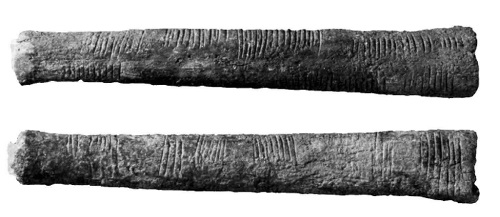
\includegraphics[width=1.0\textwidth]{img/ishango.jpg}
    \captionsetup{textfont=tiny,labelformat=empty,justification=centering}
    \caption{Hueso de Ishango (18,000{\aprox}20,000~a.e.c.)\ccbysa\cite{ishango}\\
    Un único símbolo representando la unidad.}
\end{figure}
\end{minipage}
~
\begin{minipage}{0.45\textwidth}
\begin{figure}
    \centering
    %\egyptify{0}{0}{0}{0}{0}{4}{2}
    \egone{2}\egten{4}
    \captionsetup{textfont=tiny,labelformat=empty,justification=centering}
    \caption{El número $42$ representado utilizando el sistema de numeración
    egipcio. Donde
    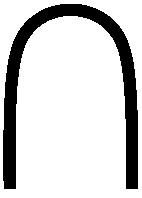
\includegraphics[scale=.05]{styles/egyptian/egypt_heel.pdf}
    equivale a 10 unidades,
    
\includegraphics[scale=.05]{styles/egyptian/egypt_stroke.pdf}
    a una unidad.}
\end{figure}
\end{minipage}

\begin{itemize}
    \item[] La suma de elementos multiplicados por su peso nos indican el número
        representado.
\end{itemize}

\end{frame}

\begin{frame}

\frametitle{Sistemas no posicionales}
\framesubtitle{Sistemas de numeración egipcio}

\begin{center}
    \tiny
    \begin{tabular}[t]{ c c c c c c c }

        El dios \emph{Heh} & Renacuajo & Dedo & Flor de loto & Cuerda
        enrollada & Grillete & Trazo\\

        \egmil{1} & \eghuntho{1} & \egtentho{1} & \egtho{1} & \eghun{1} &
        \egten{1} & \egone{1}\\

        1\,000\,000 & 100\,000 & 10\,000 & 1\,000 & 100 & 10 & 1\\

    \end{tabular}
\end{center}

\begin{itemize}
    \item ¿Cómo se representa el $2\,023$?
    \item ¿Cómo se representaría su número de \emph{DNI}?
\end{itemize}

\end{frame}

\begin{frame}

\frametitle{Sistema posicional}
\framesubtitle{¿Cómo entendemos un numeral?}

\begin{figure}
    \centering
    \includegraphics[height=0.95\textheight]{ani/sumPot-00.pdf}
    \captionsetup{textfont=tiny,labelformat=empty}
    \caption{}
\end{figure}

\end{frame}

\begin{frame}

\frametitle{Sistema posicional}
\framesubtitle{¿Cómo entendemos un numeral?}

\begin{figure}
    \centering
    \includegraphics[height=0.95\textheight]{ani/sumPot-01.pdf}
    \captionsetup{textfont=tiny,labelformat=empty}
    \caption{}
\end{figure}

\end{frame}

\begin{frame}

\frametitle{Sistema posicional}
\framesubtitle{¿Cómo entendemos un numeral?}

\begin{figure}
    \centering
    \includegraphics[height=0.95\textheight]{ani/sumPot-02.pdf}
    \captionsetup{textfont=tiny,labelformat=empty}
    \caption{}
\end{figure}

\end{frame}

\begin{frame}

\frametitle{Sistema posicional}
\framesubtitle{¿Cómo entendemos un numeral?}

\begin{figure}
    \centering
    \includegraphics[height=0.95\textheight]{ani/sumPot-03.pdf}
    \captionsetup{textfont=tiny,labelformat=empty}
    \caption{}
\end{figure}

\end{frame}

\begin{frame}

\frametitle{Sistema posicional}
\framesubtitle{¿Cómo entendemos un numeral?}

\begin{figure}
    \centering
    \includegraphics[height=0.95\textheight]{ani/sumPot-04.pdf}
    \captionsetup{textfont=tiny,labelformat=empty}
    \caption{}
\end{figure}

\end{frame}

\begin{frame}

\frametitle{Sistema posicional}
\framesubtitle{¿Cómo entendemos un numeral?}

\begin{figure}
    \centering
    \includegraphics[height=0.95\textheight]{ani/sumPot-05.pdf}
    \captionsetup{textfont=tiny,labelformat=empty}
    \caption{}
\end{figure}

\end{frame}

\begin{frame}

\frametitle{Sistema posicional}

\begin{itemize}
    \item Un número limitado de símbolos.
    \item El peso de cada ocurrencia del símbolo depende de su
        \textbf{posición}.
    \item La \textbf{\emph{base}} nos indica la cantidad de símbolos y que
        tanto más grande es cada posición con respecto a la anterior.
    \item Usualmente utilizamos los símbolos \emph(0..9) representando su
        valor usual, y si la base es mayor a 10 utilizamos letras: $ A=10,
        B=11, C=12, D=13, E=14, F=15$.
\end{itemize}

\end{frame}

\begin{frame}

\frametitle{Sistema posicional}
\framesubtitle{Expresión general: conversión decimal}

    Sea un número $N_{(b)} = X_{k}X_{k-1}...X_{2}X_{1}X_{0}$, donde cada $X_{i}$ son sus
    dígitos en base $b$. Su representación en decimal $Q_{(10)}$:

\begin{equation*}
    N_{(b)} = \displaystyle\sum_{i=0}^{k} X_{i}{\times}b^{i}
    \pause
    =
    X_{k}{\times}b^{k}+X_{k-1}{\times}b^{k-1}...
        X_{1}{\times}b^{1}+X_{0}{\times}b^{0}
    \pause
    = Q_{(10)}
\end{equation*}
\pause

Ejemplos:
\pause
\begin{itemize}
    \item
        $60_{(7)} = \pause
        6{\times}7^1+0{\times}7^0 = \pause
        42_{(10)}$\pause
    \item $2A_{(16)} = \pause
        2{\times}(16)^1+(10){\times}(16)^0 = \pause
        42_{(10)}$\pause
    \item $1120_{(3)} = \pause
        1{\times}3^3+1{\times}3^2+2{\times}3^1+0{\times}3^0 = \pause
        42_{(10)}$
\end{itemize}

\end{frame}

\begin{frame}

\title{¿Consultas?}
\maketitle

\end{frame}

\begin{frame}

\frametitle{Sistema posicional}
\framesubtitle{Conversión de decimal a otras bases}

    Para convertir $Q_{(10)}$ a su representación $N_{b}$ expresado en base
    $b$.
    \begin{enumerate}
        \item Dividir el número original por la base destino, anotando
            cociente y resto
    \item Mientras el cociente sea mayor a cero:
        \begin{itemize}
            \item Volver al paso \textbf{1} reemplazando el número original
                por el nuevo cociente.
        \end{itemize}
    \item Finalmente escribimos los dígitos de nuestro número convertido
        usando \textbf{todos los restos en orden inverso a como aparecieron}.
    \end{enumerate}

\end{frame}

\begin{frame}

\frametitle{Sistema posicional}
    \framesubtitle{Conversión de decimal a otras bases, convertir
    $1961_{(10)}$ a base 16}

    Ejemplo:
    \pause

    \begin{tabular}[t]{ l r l}

        & C & R\\

        $1961{\div}16$ & $122$ & $9$\\\pause

        $122{\div}16$ & $7$ & $10$\\\pause

        $7{\div}16$ & $0$ & $7$\\

    \end{tabular}

\pause
Entonces:
    $1961_{(10)} = 7A9_{(16)}$

\end{frame}

\begin{frame}

\frametitle{Sistema posicional}
\framesubtitle{Equivalencias entre binario, octal y hexadecimal}
\small\centering
\begin{tabular}{ | c | r | c | c | }
    \hline
    Decimal & {\centering Binario} & Octal & Hexadecimal \\
    \hline
    \hline
    0 & 000/0000 & 0 & 0 \\
    \hline
    1 & 001/0001 & 1 & 1 \\
    \hline
    2 & 010/0010 & 2 & 2 \\
    \hline
    3 & 011/0011 & 3 & 3 \\
    \hline
    4 & 100/0100 & 4 & 4 \\
    \hline
    5 & 101/0101 & 5 & 5 \\
    \hline
    6 & 110/0110 & 6 & 6\\
    \hline
    7 & 111/0111 & 7 & 7 \\
    \hline
    8 & -/1000 & - & 8 \\
    \hline
    9 & -/1001 & - & 9 \\
    \hline
    10 & -/1010 & - & A \\
    \hline
    11 & -/1011 & - & B \\
    \hline
    12 & -/1100 & - & C \\
    \hline
    13 & -/1101 & - & D \\
    \hline
    14 & -/1110 & - & E \\
    \hline
    15 & -/1111 & - & F \\
    \hline
\end{tabular}

\end{frame}

\begin{frame}

\frametitle{Sistema posicional}
\framesubtitle{Equivalencias entre binario, octal y hexadecimal}

Ejemplo:

\begin{figure}
    \centering
    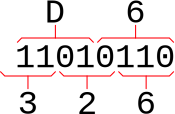
\includegraphics[height=0.75\textheight]{img/convBin.pdf}
    \captionsetup{textfont=tiny,labelformat=empty}
    \caption{}
\end{figure}

\end{frame}

\begin{frame}

    \frametitle{Temario}

\begin{itemize}

    \item Números y numerales.

    \item Sistemas no posicionales.

    \item Sistemas posicionales:
    \begin{itemize}
        \item Conversión entre bases.
    \end{itemize}

\end{itemize}
\end{frame}

\begin{frame}

\title{¿Consultas?}
\maketitle

\end{frame}

\newcounter{lastPage}
\setcounter{lastPage}{\number\value{page}}

\begin{frame}%[allowframebreaks]

\frametitle{Atribuciones}

\bibliographystyle{abbrv}
\setbeamertemplate{bibliography item}{\insertbiblabel}
\tiny
\bibliography{refimg}
\end{frame}

\setcounter{page}{\number\value{lastPage}}

\end{document}
